% ****** Start of file apssamp.tex ******
%
%   This file is part of the APS files in the REVTeX 4.1 distribution.
%   Version 4.1r of REVTeX, August 2010
%
%   Copyright (c) 2009, 2010 The American Physical Society.
%
%   See the REVTeX 4 README file for restrictions and more information.
%
% TeX'ing this file requires that you have AMS-LaTeX 2.0 installed
% as well as the rest of the prerequisites for REVTeX 4.1
%
% See the REVTeX 4 README file
% It also requires running BibTeX. The commands are as follows:
%
%  1)  latex apssamp.tex
%  2)  bibtex apssamp
%  3)  latex apssamp.tex
%  4)  latex apssamp.tex
%
\documentclass[%
 reprint,
%superscriptaddress,
%groupedaddress,
%unsortedaddress,
%runinaddress,
%frontmatterverbose, 
%preprint,
%showpacs,preprintnumbers,
%nofootinbib,
%nobibnotes,
%bibnotes,
 amsmath,amssymb,
 aps,
%pra,
%prb,
%rmp,
%prstab,
%prstper,
%floatfix,
]{revtex4-1}

\usepackage{graphicx}% Include figure files
\usepackage{dcolumn}% Align table columns on decimal point
\usepackage{bm}% bold math
%\usepackage{hyperref}% add hypertext capabilities
%\usepackage[mathlines]{lineno}% Enable numbering of text and display math
%\linenumbers\relax % Commence numbering lines

%\usepackage[showframe,%Uncomment any one of the following lines to test 
%%scale=0.7, marginratio={1:1, 2:3}, ignoreall,% default settings
%%text={7in,10in},centering,
%%margin=1.5in,
%%total={6.5in,8.75in}, top=1.2in, left=0.9in, includefoot,
%%height=10in,a5paper,hmargin={3cm,0.8in},
%]{geometry}

\begin{document}

\preprint{APS/123-QED}

\title{Difracción de electrones}% Force line breaks with \\
\thanks{A footnote to the article title}%

\author{Ann Author}
 \altaffiliation[Also at ]{Departamento de Física, Universidad de los Andes}%Lines break automatically or can be forced with \\
\author{Sergio Iv\'an Rey}%
 \email{si.rey1826@uniandes.edu.co}
\affiliation{%
 Departamento de Física, Universidad de los Andes
}%

\date{13/8/2015}% It is always \today, today,
             %  but any date may be explicitly specified

\begin{abstract}
En este laboratorio verificamos cualitativamente la dualidad onda-partícula del electrón y cuantificamos la difracción de un rayo de electrones pasando a través de un blanco de grafito. Con esta cuantificación pudimos calcular las distancias interplanares de los cristales de grafito. Obtuvimos los resultados $d1 = x \pm err$ y $d2 = y \pm err$, lo cual se acerca con gran exactitud a los valores reales, teniendo errores de únicamente $ x1\%$ y $ x2\%$. De la misma manera se pudo obtener un valor considerablemente acertado de la constante de Planck, $ h = z \pm err $, lo cual solo está alejado del valor real un $ planck\% $. Los errores obtenidos se atribuyen principalmente a la precisión de los elementos usados para hacer las mediciones, además del ancho natural de los círculos de difracción.
\end{abstract}


\keywords{Difracción de electrones. Distancias interplanares. Constante de Planck}%Use showkeys class option if keyword
                              %display desired
\maketitle

%\tableofcontents

\section{\label{sec:level1}Introducci\'on}
Uno de las consecuencias más imporatnes de la mecánica cuántica es la interpretación de los fenómenos físicos poco intuitivos con partículas como parte de una dualidad onda-partícula. Ésta dualidad hace referencia al comportamiento de la materia como onda en ciertas circustancias, y como partícula en otras. Un caso particular del comportamiento de una partícula como onda puede ser presenciada con el electrón. Al lanzar un haz coherente de electrones contra un blanco con las características adecuadas, se puede apreciar un patrón de difracción al igual que en una onda normal.\\

Para cuantificar la difracción de electrones, es muy útil saber cuantificar la difracción en una onda común. Supóngase entonces que se hace incidir una onda de longitud de onda $\lambda$, a un ángulo $\theta$ sobre un cristal con distancia interplanar $d$ como se muestra en la figura \ref{fig:difraccion}. Parte de la onda se reflejará en el primer plano, y parte de la onda se reflejará en el segundo plano. Si se asume la distancia interplanar lo suficientemente pequeña para omitir los efectos de refracción, la onda que pasa al segundo plano volverá a encontrarse con la que se refleja en el primero. Sin embargo, debido al camino de más que ha recorrido, habrá una diferencia de fase que será importante para determinar si estas ondas se anulan o se refuerzan.\\ 


\begin{figure}[h]
\caption{Difracción de Brag}
\centering
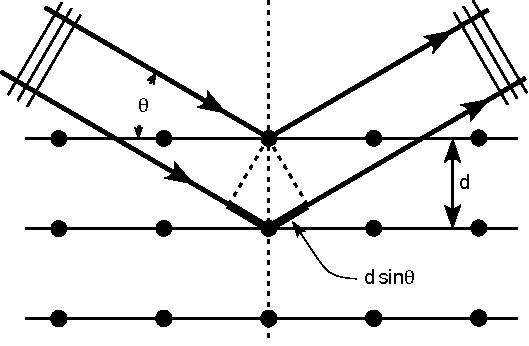
\includegraphics[width=0.30\textwidth]{difraction}
\label{fig:difraccion}
\end{figure}

De la figura \ref{fig:difraccion} es claro ver que la diferencia de caminos es de $d\sin{\theta}$. Con esto, y sabiendo que la longitud de onda del rayo incidente es $\lambda$, se puede calcular la diferencia de fase entre las dos ondas. Esta diferencia está dada por la ecuación\ref{equation:phase} a continuación.\\

\begin{equation}
\delta = \frac{(2\pi)(d\sin{\theta}}{\lambda} = \frac{2\pi d\sin{\theta}}{\lambda}
\label{equation:phase}
\end{equation}

Dado esto, si asumimos una onda sinusoidal normal, ambas ondas se anularán cuando su diferencia de fase sea $\delta = \pi$ y sea $\delta = 2\pi$. Claramente habrá interferencia constructiva y destructiva respectivamente para ángulos mayores si se agrega $2\pi$ a cada desfase. Sin embargo, en este caso, para poder apreciar un buen patrón de difracción, consideramos que la longitud de onda de la onda incidente es del orden de magnitud de la distancia interplanar, por lo que se omitirán dichos casos. Además, si la onda se observa a una distancia $L$ del blanco en dirección perpendicular al plano del blanco, y a una distancia $R$ del blanco en dirección paralela a éste, asumiendo incidencia casi normal, es decir, $\theta \approx 0$, se tiene $\sin{\theta} \approx \frac{R}{L}$. Con todo esto, observaremos un patrón de interferencia constructiva que caracterizará el patrón de difracción cuando se cumpla la condición dada en la ecuación \ref{equation:mas}.\\

\begin{equation}
\frac{d\sin{\theta}}{\lambda} = \frac{dR}{L\lambda} = 1
\label{equation:mas}
\end{equation}

Ahora, sabiendo cuantificar la difracción para una onda normal, se puede caracterizar también la difracción de un haz de electrones. Para esto, solo es necesario tener en cuenta la relación de De Broglie para obtener la longitud de onda de un electrón libre con una energía $E$ determinada. La longitud de onda será entonces de la forma:\\

\begin{equation}
\lambda = \frac{p}{h} = \frac{\sqrt{2mE}}{h}
\label{equation:lambda}
\end{equation}

Donde claramente $h$ es la constante de Planck y $m$ es la masa del elctrón. Si asumimos además que cada electrón fue acelerado por un potencial eléctrico $V$, la ecuación \ref{equation:lambda} se reduce a:\\

\begin{equation}
\lambda = \frac{p}{h} = \frac{\sqrt{2meV}}{h}
\label{equation:lambda2}
\end{equation}

Ahora, la condición para el máximo en el patrón de difracción de electrones está dado por la unión de las ecuaciones \ref{equation:mas} y \ref{equation:lambda2}. En este caso, quedamos con la ecuación final para cuantificar la difracción de electrones: 

 \begin{equation}
\frac{dR}{L} = \frac{p}{h} = \frac{\sqrt{2meV}}{h}
\label{equation:lambda2}
\end{equation}

En este experimento tomaremos un blanco hecho de grafito. El grafito está compuesto de cristales pequeños irregularmente distribuidos. Estos cristales tienen celda unitaria hexagonal, por lo que habrán dos distancias interplanares importantes. Éstas distancias se muestran en la figura \ref{fig:carbono}. Estas distancias interplanares se sabe que tienen los valores:\\

\begin{equation}
d1 = ; d2 = 
\label{equation:carbono}
\end{equation}

%poner imagen del cristal de carbono.

Dado que se mandará un haz de electrones de simetría cilíndrica contra el blanco de grafito, el patrón de difraccoión tendrá también simetría cilíndrica, es decir, observaremos círculos como patrones. En este sentido es mejor escribir la ecuación \ref{equation:lambda2} en términos del diámetro $D = 2R$ de los círculos observados:\\

 \begin{equation}
\frac{dD}{2L} = \frac{\sqrt{2meV}}{h}
\label{equation:final}
\end{equation} 



\section{\label{sec:level1}Montaje experimental}


\section{\label{sec:level1}Resultados y An\'alisis}

\subsection{\label{sec:level2}Circuito RC}


\subsection{\label{sec:level2}Circuito RLC Forzado}


\begin{table}[h!]
\centering
 \begin{tabular}{|c|c|c|} 
 \hline
 $Frecuencia$ (Hz) & $V_{pp}$ (V) & $V_rms$ \\ [0.5ex] 
 \hline\hline
16.3 &		12.6 &		4.37\\
16.5 &		12.5 &		4.35\\
16.7 &		12.4 &		4.3\\
17.0 &		12 &		4.18\\
17.5 &		11.1 &		3.85\\
18.0 &		9.84 &		3.41\\
16.1 &		12.5 &		4.36\\
16.9 &		12.4 &		4.3\\
15.6 &		12 &		4.16\\
15.2 &		11.4 &		3.93\\
14.5 &		10 &		3.42\\
14.0 &		9.28 &		3.19\\
13.0 &		7.84 &		2.72\\
12.0 &		6.96 &		2.37\\
19.0 &		7.60 &		2.62\\
20.0 &		5.76 &		1.98\\
[1ex] 
 \hline
 \end{tabular}
 \caption{Datos de curva de resonancia RLC.}
 \label{table:resonancia}
\end{table}
 citation in text uses the command \verb+\cite{#1}+ or
\verb+\onlinecite{#1}+ and refers to an entry in the bibliography. 
An entry in the bibliography is a reference to another document.

\subsubsection{Citations}
Because REV\TeX\ uses the \verb+natbib+ package of Patrick Daly, 




 


 


\section{\label{sec:level1}Conclusiones}



\subsection{\label{sec:citeref}Citations and References}
A citation in text uses the command \verb+\cite{#1}+ or
\verb+\onlinecite{#1}+ and refers to an entry in the bibliography. 
An entry in the bibliography is a reference to another document.

\subsubsection{Citations}
Because REV\TeX\ uses the \verb+natbib+ package of Patrick Daly, 
the entire repertoire of commands in that package are available for your document;
see the \verb+natbib+ documentation for further details. Please note that
REV\TeX\ requires version 8.31a or later of \verb+natbib+.

\paragraph{Syntax}
The argument of \verb+\cite+ may be a single \emph{key}, 
or may consist of a comma-separated list of keys.
The citation \emph{key} may contain 
letters, numbers, the dash (-) character, or the period (.) character. 
New with natbib 8.3 is an extension to the syntax that allows for 
a star (*) form and two optional arguments on the citation key itself.
The syntax of the \verb+\cite+ command is thus (informally stated)
\begin{quotation}\flushleft\leftskip1em
\verb+\cite+ \verb+{+ \emph{key} \verb+}+, or\\
\verb+\cite+ \verb+{+ \emph{optarg+key} \verb+}+, or\\
\verb+\cite+ \verb+{+ \emph{optarg+key} \verb+,+ \emph{optarg+key}\ldots \verb+}+,
\end{quotation}\noindent
where \emph{optarg+key} signifies 
\begin{quotation}\flushleft\leftskip1em
\emph{key}, or\\
\texttt{*}\emph{key}, or\\
\texttt{[}\emph{pre}\texttt{]}\emph{key}, or\\
\texttt{[}\emph{pre}\texttt{]}\texttt{[}\emph{post}\texttt{]}\emph{key}, or even\\
\texttt{*}\texttt{[}\emph{pre}\texttt{]}\texttt{[}\emph{post}\texttt{]}\emph{key}.
\end{quotation}\noindent
where \emph{pre} and \emph{post} is whatever text you wish to place 
at the beginning and end, respectively, of the bibliographic reference
(see Ref.~[\onlinecite{witten2001}] and the two under Ref.~[\onlinecite{feyn54}]).
(Keep in mind that no automatic space or punctuation is applied.)
It is highly recommended that you put the entire \emph{pre} or \emph{post} portion 
within its own set of braces, for example: 
\verb+\cite+ \verb+{+ \texttt{[} \verb+{+\emph{text}\verb+}+\texttt{]}\emph{key}\verb+}+.
The extra set of braces will keep \LaTeX\ out of trouble if your \emph{text} contains the comma (,) character.

The star (*) modifier to the \emph{key} signifies that the reference is to be 
merged with the previous reference into a single bibliographic entry, 
a common idiom in APS and AIP articles (see below, Ref.~[\onlinecite{epr}]). 
When references are merged in this way, they are separated by a semicolon instead of 
the period (full stop) that would otherwise appear.

\paragraph{Eliding repeated information}
When a reference is merged, some of its fields may be elided: for example, 
when the author matches that of the previous reference, it is omitted. 
If both author and journal match, both are omitted.
If the journal matches, but the author does not, the journal is replaced by \emph{ibid.},
as exemplified by Ref.~[\onlinecite{epr}]. 
These rules embody common editorial practice in APS and AIP journals and will only
be in effect if the markup features of the APS and AIP Bib\TeX\ styles is employed.

\paragraph{The options of the cite command itself}
Please note that optional arguments to the \emph{key} change the reference in the bibliography, 
not the citation in the body of the document. 
For the latter, use the optional arguments of the \verb+\cite+ command itself:
\verb+\cite+ \texttt{*}\allowbreak
\texttt{[}\emph{pre-cite}\texttt{]}\allowbreak
\texttt{[}\emph{post-cite}\texttt{]}\allowbreak
\verb+{+\emph{key-list}\verb+}+.

\end{document}
%
% ****** End of file apssamp.tex ******
